\section{Prototyp zapojenia pomocou breadboardu}

Na otestovanie správnosti a funkčnosti kódu bol zostavený model systému na breadboarde obr.\ref{OBRAZOK 1.4}. Systém po niekoľkých iteráciách softwaru a hardwaru fungoval s vysokou presnosťou a bolo možné ho vyladiť podľa potrieb užívateľa. Na ovládanie prvej verzie ovládača hlasitosti sme použili Arduino UNO ktorého sériový port a vykresľovanie meraných veličín nám veľmi uľahčili proces vylepšovania kódu.

\begin{figure}[!tbh]
\centering
\fbox{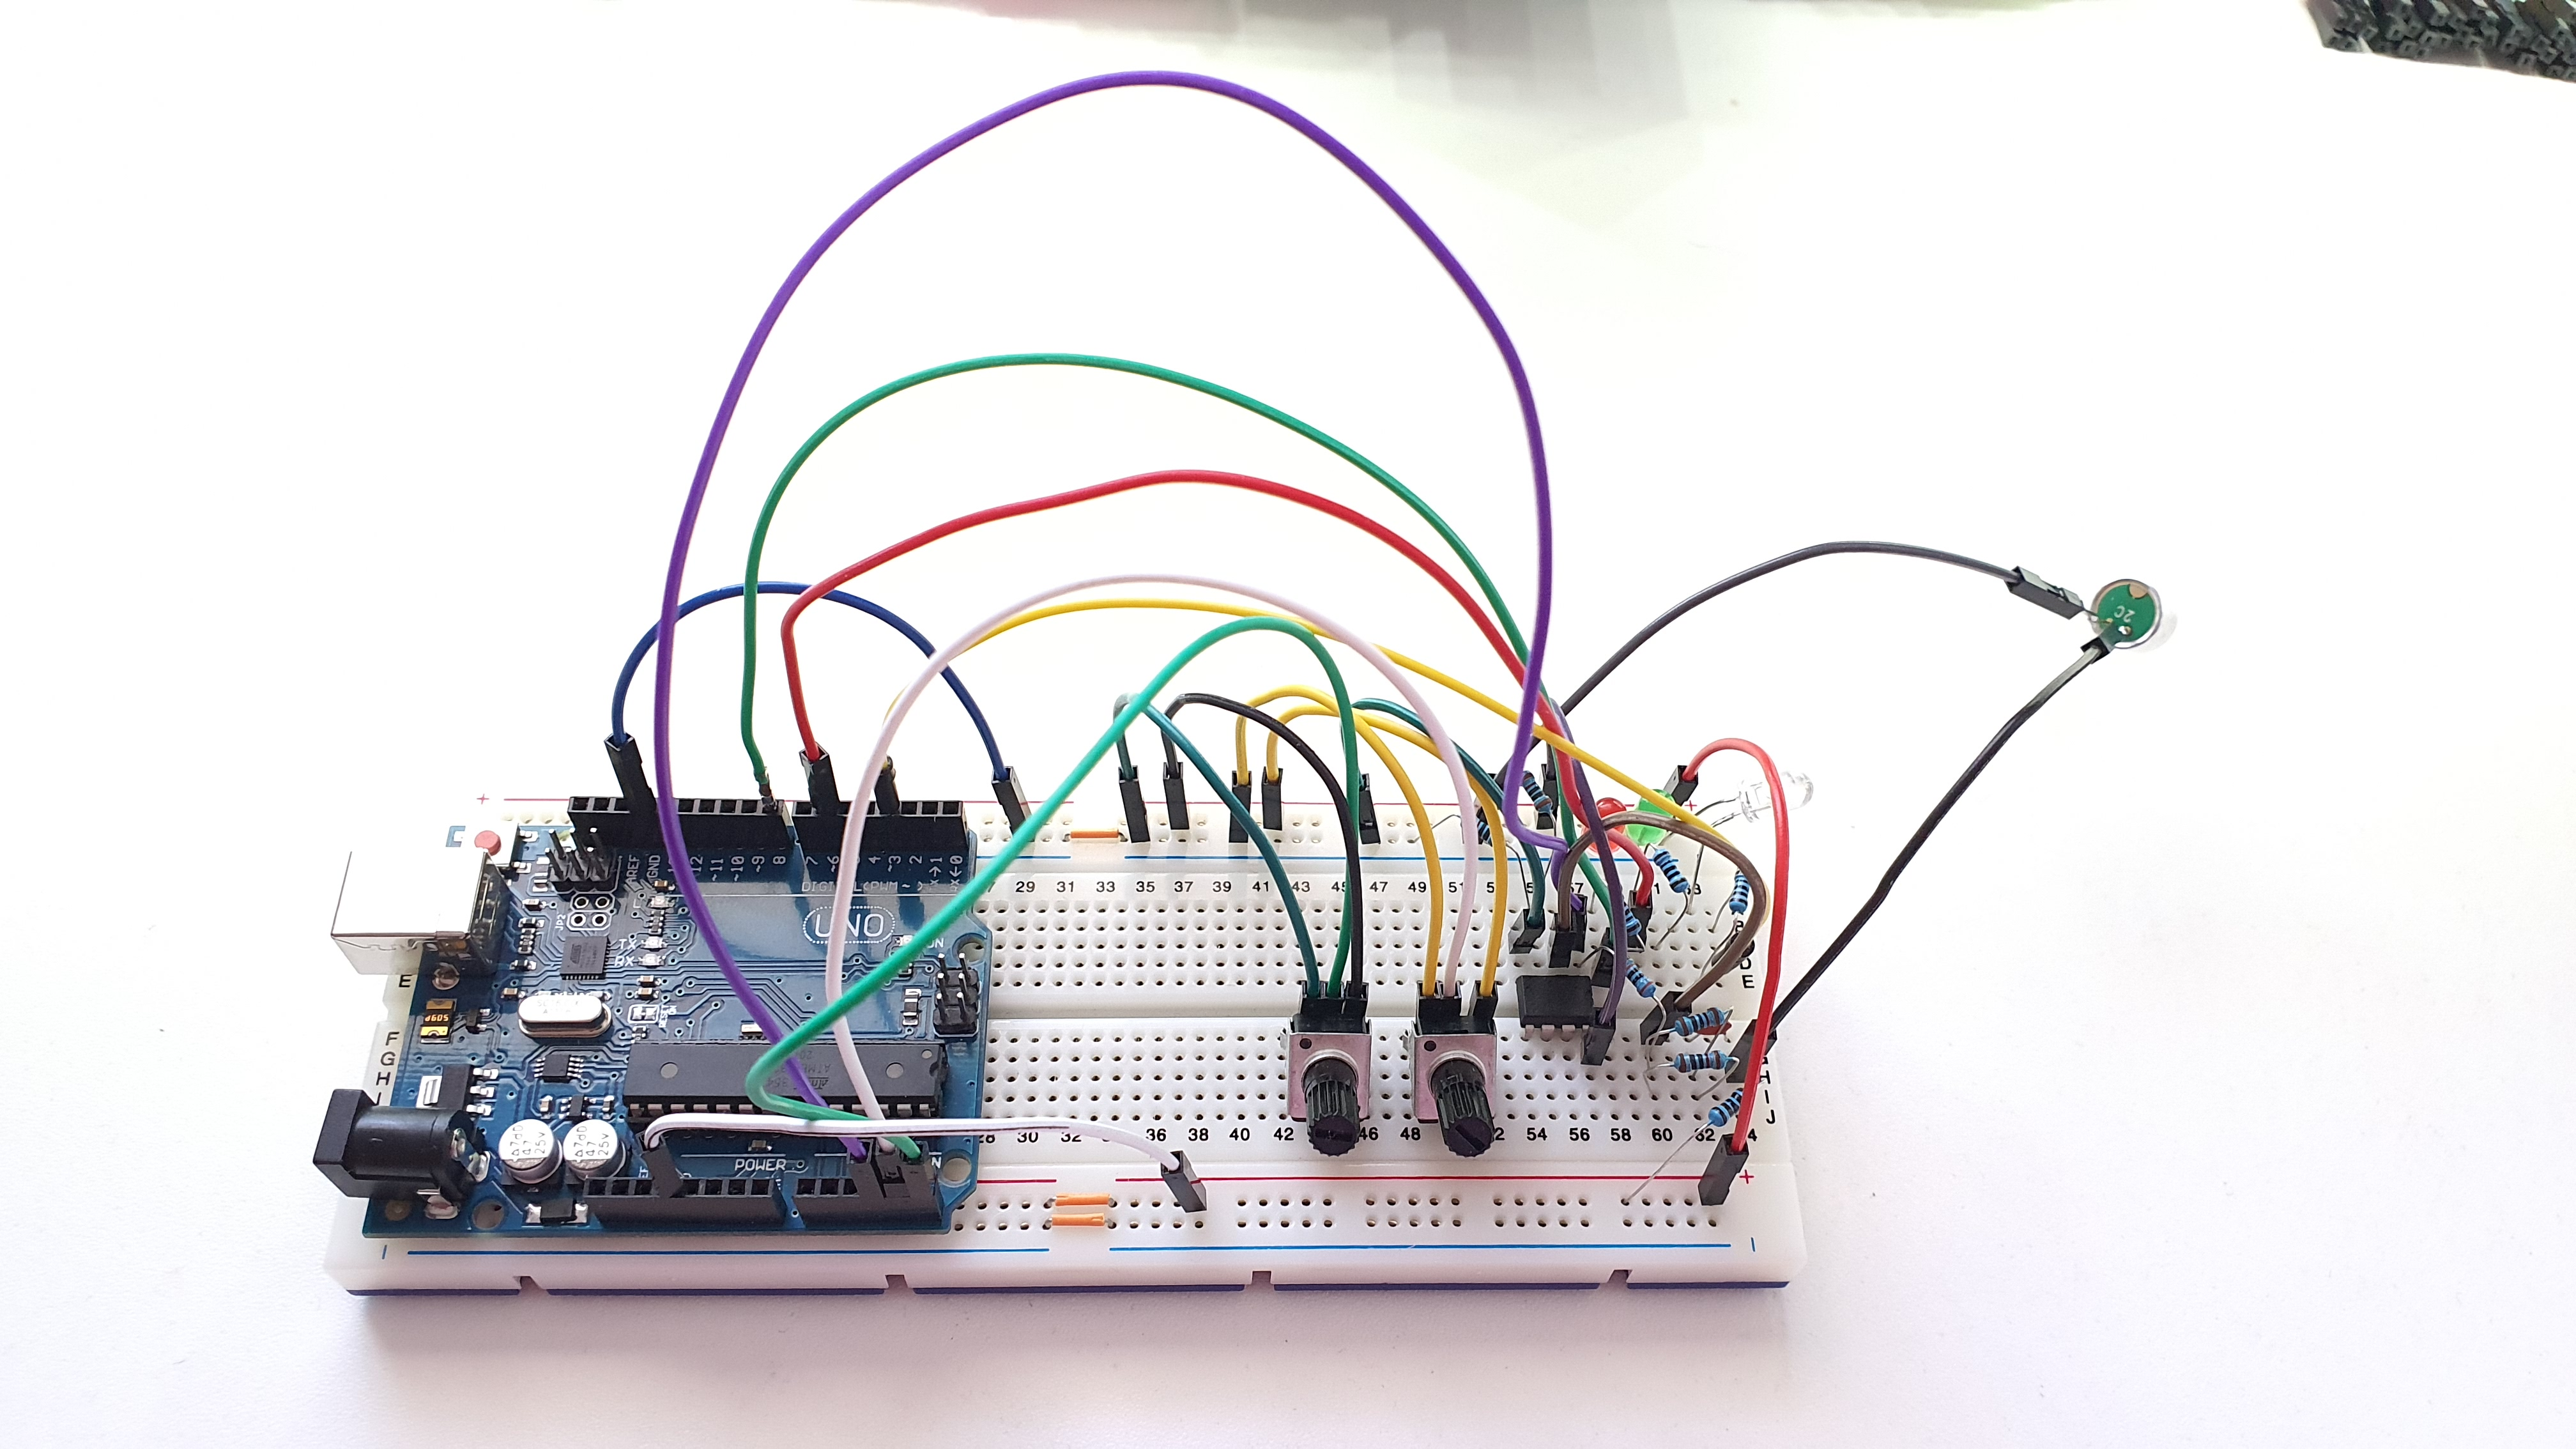
\includegraphics[width=12cm]{obr/breaduno2.jpg}}
\caption{Zapojenie na breadboarde.}\label{OBRAZOK 1.4}
\end{figure}

\begin{figure}[!tbh]
\centering
\fbox{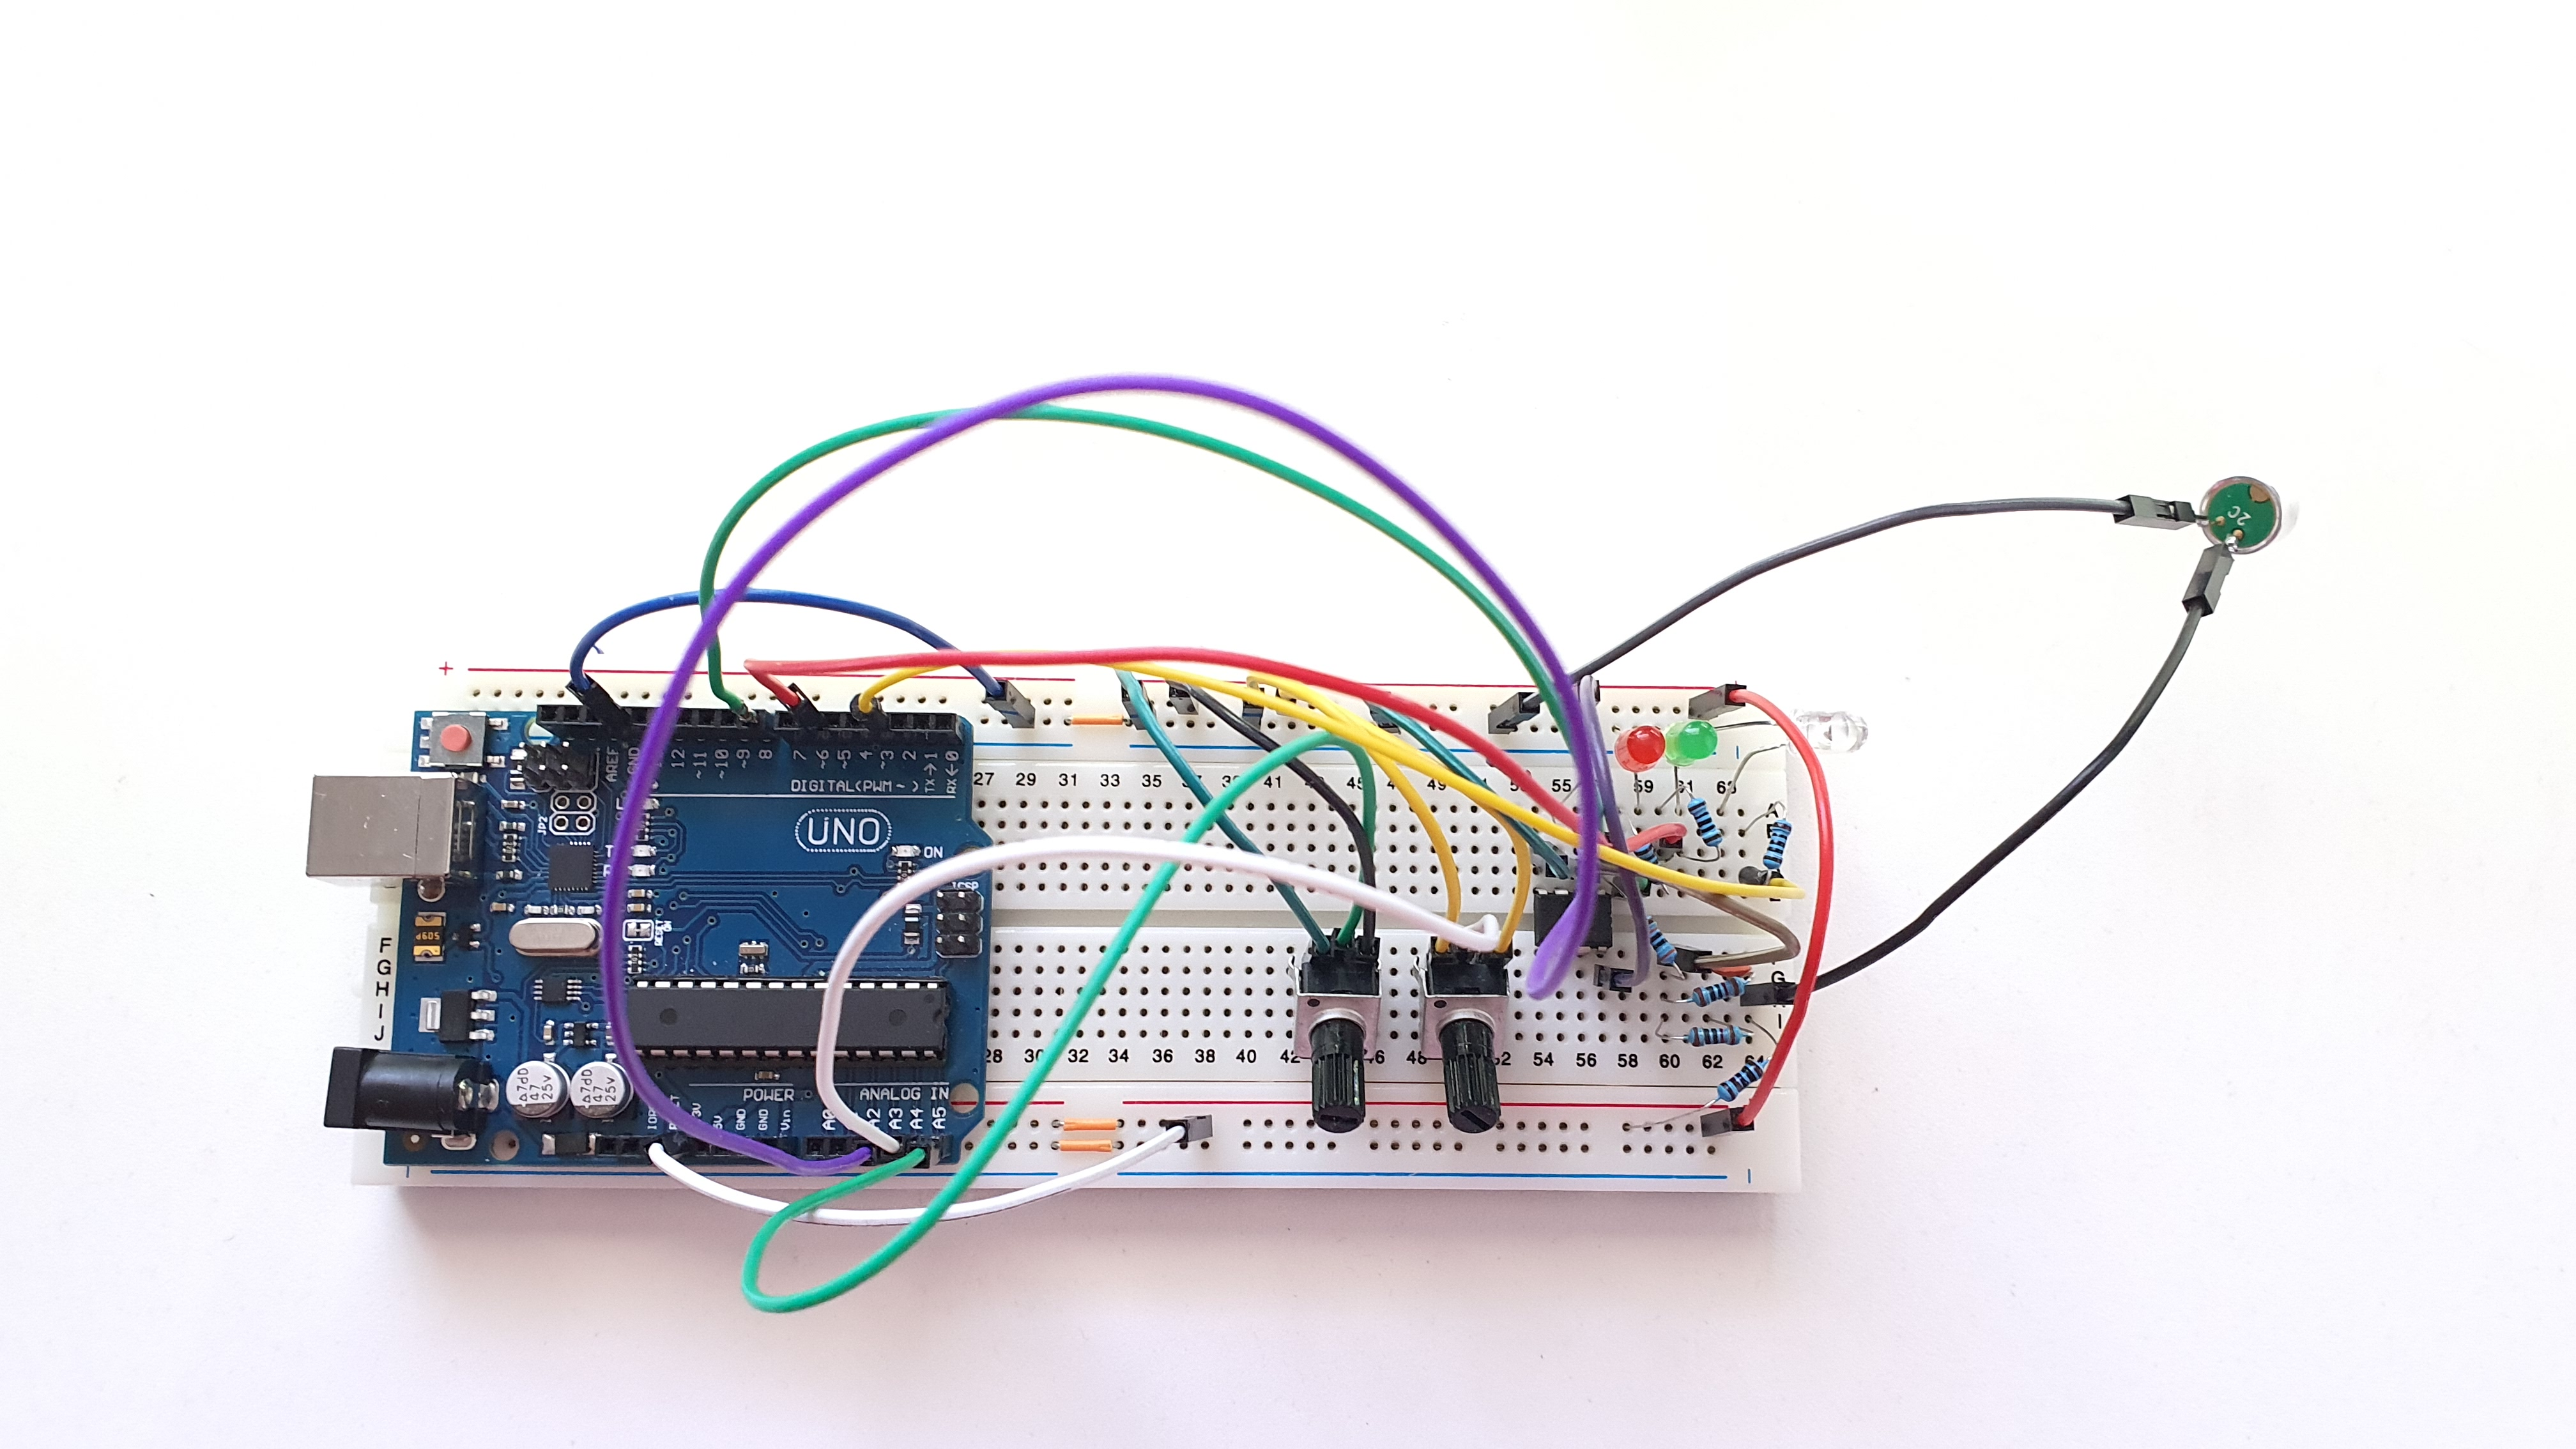
\includegraphics[width=12cm]{obr/breadunohorepohlad.jpg}}
\caption{Zapojenie na breadboarde.}\label{OBRAZOK 1.4}
\end{figure}

